\documentclass[conference]{IEEEtran}
\IEEEoverridecommandlockouts
\usepackage{cite}
\usepackage{amsmath,amssymb,amsfonts}
\usepackage{graphicx}
\usepackage{textcomp}
\usepackage{xcolor}
\usepackage{booktabs}
\usepackage{multirow}
\usepackage{url}
\usepackage{microtype}
\usepackage{tikz}
\usetikzlibrary{positioning,arrows.meta,fit,backgrounds}
\usepackage{listings}
\lstset{
  basicstyle=\ttfamily\scriptsize,
  breaklines=true,
  frame=single,
  frameround=tttt,
  belowskip=0pt,
  aboveskip=4pt
}

\begin{document}

\title{SensorWF: A FAIR Generalizable Workflow Framework\\for Multi-Domain Scientific Time-Series Analysis}

\author{
  \IEEEauthorblockN{Author Name\textsuperscript{1},
                    Author Name\textsuperscript{2}}
  \IEEEauthorblockA{\textsuperscript{1}\textit{Department, Institution, City, Country}\\
                    \textsuperscript{2}\textit{Department, Institution, City, Country}\\
                    email@example.com}
}

\maketitle

\begin{abstract}
Scientific sensor data analyses across diverse domains -- spacecraft telemetry,
biomedical signals, and atmospheric measurements -- share a common analytical
skeleton: ingest raw data, assess quality, engineer features, inject ground-truth
faults, evaluate detectors, annotate semantically, and record provenance. Yet
pipelines in each domain are typically published as monolithic, domain-specific
scripts whose assumptions are implicit and whose components cannot be reused
across disciplines. We present \textbf{SensorWF}, a FAIR-annotated, generalizable
computational workflow framework for scientific time-series analysis. SensorWF
decomposes the end-to-end analysis pipeline into seven formally specified modules
(M1--M7) with typed input/output contracts and a machine-readable component
registry. A \emph{domain adapter} pattern makes M1 the only domain-specific
component, while M2--M7 remain fully reusable. We validate SensorWF across three
scientifically distinct domains: (i) spacecraft telemetry from the KISPE
Satellite Learning Laboratory (SATLL), (ii) ambulatory ECG recordings from the
MIT-BIH Arrhythmia Database, and (iii) hourly meteorological observations from
the Jena Climate Dataset. Across all three domains, four ML anomaly detectors
are evaluated against systematically injected faults; the Autoencoder achieves
aggregate AUC-ROC of 0.705 (satellite), 0.794 (ECG), and 0.803 (climate).
Runtime PROV-O/ProvONE provenance traces and domain-specific OWL ontologies are
emitted as first-class workflow outputs. All workflow code, component registry,
ontology artefacts, and result datasets are released as an open scientific object.
\end{abstract}

\begin{IEEEkeywords}
computational workflows, FAIR principles, domain adaptation, sensor analytics,
anomaly detection, PROV-O, ProvONE, knowledge graph, reproducibility
\end{IEEEkeywords}

%% =========================================================
\section{Introduction}
\label{sec:intro}
%% =========================================================

Scientific disciplines that rely on continuous sensor streams -- from satellite
telemetry and biomedical monitoring to environmental observation -- face a common
set of computational challenges. Raw sensor data must be ingested, corrected
for artefacts, transformed into analysis-ready feature representations, and
evaluated against ground-truth labels for anomaly detection or classification.
Each stage encodes domain assumptions about sampling rates, quality thresholds,
fault morphologies, and evaluation protocols that are rarely made explicit or
machine-readable.

Despite this shared structure, pipelines across these domains are almost always
developed in isolation as monolithic, domain-specific scripts. The resulting
fragmentation prevents reuse, makes cross-domain comparisons unreliable, and
renders post-publication audit practically impossible. The eScience and
open-science communities have called for pipelines to be treated as first-class
scientific objects whose provenance can be traced, shared, and reused
\cite{wilkinson2016fair,garijo2022fair}.

This paper presents \textbf{SensorWF} (\emph{Generalizable FAIR Sensor Analytics
Workflow}), a framework that addresses this gap. SensorWF makes four specific
contributions:

\begin{enumerate}
  \item \textbf{A generalizable seven-module architecture.} SensorWF decomposes
    sensor data analysis into modules M1--M7, each with typed I/O contracts and
    explicit scientific assumptions. The \emph{domain adapter} pattern isolates
    domain-specificity in M1, making M2--M7 fully reusable across disciplines.
  \item \textbf{A machine-readable component registry.} A structured
    \texttt{components.json} document formally describes every module: inputs,
    outputs, configuration parameters, domain tags, and ProvONE URI, enabling
    automated composition and discovery.
  \item \textbf{Runtime provenance and semantic annotation.} SensorWF emits
    PROV-O/ProvONE Turtle provenance for every execution, and maps ML detector
    evidence to domain OWL ontologies (SSN/SOSA-aligned), producing
    SPARQL-queryable knowledge graphs.
  \item \textbf{Cross-domain validation.} We validate SensorWF on three
    well-established benchmark datasets: KISPE SATLL (satellite telemetry),
    MIT-BIH Arrhythmia Database (biomedical ECG), and the Jena Climate Dataset
    (atmospheric science), demonstrating that a single workflow framework can
    serve scientifically distinct domains.
\end{enumerate}

%% =========================================================
\section{Background and Related Work}
\label{sec:background}
%% =========================================================

\subsection{FAIR Computational Workflows}

The FAIR principles -- Findable, Accessible, Interoperable, Reusable -- were
originally formulated for scientific data \cite{wilkinson2016fair} and extended
to computational workflows \cite{garijo2022fair}. FAIR workflows expose typed
module specifications, machine-readable provenance, and explicit scientific
assumptions. Mitchell et al.\ \cite{mitchell2022fair} demonstrate PROV-O
provenance for epidemiological pipelines. WorkflowHub \cite{wilkinson2025workflowhub}
operationalises workflow registration. Rossi et al.\ \cite{rossi2025openeo}
integrate provenance into the openEO Earth Observation platform. SensorWF
complements this work by targeting \emph{multi-domain generalizability} through
an adapter pattern and a structured component registry, rather than
domain-specific pipelines.

\subsection{Domain Adapter Patterns in Scientific Computing}

Domain adaptation -- separating domain-specific components from reusable
algorithmic cores -- is well established in software engineering. In scientific
workflows this pattern appears in tools such as the Galaxy platform
\cite{afgan2018galaxy} and in time-series toolkits like TSFEL \cite{barandas2020tsfel}.
SensorWF adopts this pattern as an explicit architectural principle: the domain
adapter (M1) is the only component that changes between domains, while M2--M7
consume a standardised DataFrame schema regardless of origin.

\subsection{Anomaly Detection in Sensor Data}

Across target domains, anomaly detection baselines are established. For spacecraft
telemetry, Hundman et al.\ \cite{hundman2018detecting} established LSTM-based
detection on NASA SMAP/MSL; the OPS-SAT benchmark \cite{ruszczak2025opssat}
provides a public reference. For biomedical ECG, the MIT-BIH Arrhythmia Database
\cite{moody2001mitbih} is the canonical benchmark, with detectors ranging from
rule-based to deep autoencoder approaches \cite{kachuee2018ecgclass}. For climate
data, anomaly detection from the Jena Climate Dataset \cite{jena_climate} is
widely studied with autoregressive and isolation-based methods
\cite{martinez2020climate}. Wu and Keogh \cite{wu2022benchmarks} demonstrate
that many time-series benchmarks are confounded by single-axis difficulty scaling,
motivating SensorWF's multi-parameter tier design.

%% =========================================================
\section{SensorWF Framework Architecture}
\label{sec:architecture}
%% =========================================================

\subsection{Design Principles}

SensorWF is structured around four principles:

\textbf{Adapter isolation.} All domain-specific logic is confined to M1 via the
\texttt{DomainAdapter} abstract interface. Each adapter implements \texttt{load()},
\texttt{get\_quality\_config()}, \texttt{get\_feature\_config()},
\texttt{get\_ontology\_path()}, and \texttt{get\_fault\_types()}, providing
complete configuration for all downstream modules. Switching domains requires only
providing a new adapter.

\textbf{Explicit I/O contracts.} Every module declares typed input and output
ports matching the ProvONE \texttt{provone:Program}/\texttt{provone:InPort}/
\texttt{provone:OutPort} pattern \cite{missier2013provone}. Contracts are encoded
both in the static workflow specification (\texttt{workflow\_spec.ttl}) and in the
\texttt{components.json} registry.

\textbf{Scientific assumption transparency.} Domain assumptions -- sampling
rates, quality thresholds, window sizes, fault morphologies -- are recorded as
\texttt{sensorwf:hasAssumption} predicates in both the static specification and
runtime provenance trace, making them SPARQL-queryable and auditable.

\textbf{Reproducibility by design.} All randomness flows from a single seeded
generator chain (\texttt{seed = 42}). Running the domain entry point twice
produces bit-identical clean data, injection summaries, detection metrics, and
KG artefacts.

\subsection{Component Registry}

The \texttt{components.json} file is SensorWF's machine-readable component
registry. Each entry records: module \texttt{id}, \texttt{name},
\texttt{version}, \texttt{domain\_tags} (e.g., \texttt{"satellite\_telemetry"},
\texttt{"biomedical\_ecg"}, \texttt{"atmospheric\_climate"}), typed \texttt{inputs}
and \texttt{outputs} with format annotations, \texttt{config\_params} with defaults,
scientific \texttt{assumptions}, and \texttt{provone\_uri}. Table~\ref{tab:registry}
summarises all seven modules.

\begin{table}[t]
\caption{SensorWF Component Registry Summary}
\label{tab:registry}
\centering
\scriptsize
\setlength{\tabcolsep}{3pt}
\begin{tabular}{@{}lp{1.9cm}p{3.8cm}@{}}
\toprule
\textbf{ID} & \textbf{Module} & \textbf{Key Assumptions / Domain Tags} \\
\midrule
M1 & Data Ingestion     & Adapter-specified format; all domains \\
M2 & Quality Assessment & Stuck $\le$3 unique; gap mult.\,3--10$\times$; all domains \\
M3 & Feature Engineering& Window size adapter-configurable (15--100 samples); all domains \\
M4 & Fault Injection    & 6--18 morphologies; amplitude/duration tiering; all domains \\
M5 & Anomaly Detection  & Train on 60\% prefix; threshold at 99th percentile; all domains \\
M6 & Semantic Annotation& SSN/SOSA-aligned OWL per domain; all domains \\
M7 & Provenance Export  & PROV-O/ProvONE Turtle; UTC ISO\,8601; all domains \\
\bottomrule
\end{tabular}
\end{table}

\subsection{Module Descriptions}

\textbf{M1 -- Data Ingestion.} The \texttt{DomainAdapter} interface provides a
\texttt{load(path)} method returning a standardised DataFrame with mandatory columns
\texttt{timestamp}, \texttt{elapsed\_s}, and one or more signal channels. Three
concrete adapters are provided: \texttt{SatelliteAdapter} (SCOTTI v2 hex-encoded
telemetry), \texttt{ECGAdapter} (MIT-BIH CSV at 360\,Hz, downsampled to 50\,Hz),
and \texttt{ClimateAdapter} (Jena CSV at 10-minute resolution, 14 channels).

\textbf{M2 -- Quality Assessment.} Domain-agnostic quality checks driven by the
adapter's \texttt{get\_quality\_config()} dictionary: NaN rates, stuck-sensor
detection ($\le k$ unique values in a window), timing regularity ($>n\times$ expected
interval), per-channel Z-score flags, and optional linear-trend detection. Outputs
a quality report JSON and a clean DataFrame.

\textbf{M3 -- Feature Engineering.} Constructs four feature families: (i) raw
channel values; (ii) first-order differences; (iii) packet-interval features from
\texttt{elapsed\_s}; and (iv) rolling mean and standard deviation (window from
\texttt{get\_feature\_config()}). The resulting feature matrix is consumed by M5.

\textbf{M4 -- Fault Injection.} Reads the adapter's \texttt{get\_fault\_types()}
list and applies each morphology across three difficulty tiers (easy, medium, hard),
simultaneously scaling amplitude, duration, and channel spread. With 2 variants per
(type, tier) combination, M4 produces $N \times 3 \times 2$ labelled injection
sessions where $N$ is the number of fault types.

\textbf{M5 -- Anomaly Detection.} Trains four ML detectors on the first 60\% of
the clean session: (i) Z-score with MAD-robust fusion; (ii) RobustRollingZScore
with CUSUM persistence; (iii) IsolationForest with a three-member rotation ensemble
\cite{liu2008isolation}; and (iv) a multi-scale MLP Autoencoder with denoising
\cite{malhotra2016lstm}. All thresholds are the 99th percentile of training scores.
Per-fault-type and aggregate metrics (accuracy, FPR, recall, F1, AUC-ROC) are
reported by difficulty tier.

\textbf{M6 -- Semantic Annotation.} Maps ML detector evidence to a domain-specific
OWL ontology (path from \texttt{get\_ontology\_path()}), building a knowledge graph
of OWL class instances, anomaly tags, feature nodes, and per-instance evidence. For
IsolationForest, \texttt{if:featureImportance} edges link feature nodes to ontology
classes. Outputs RDF/Turtle and GraphML.

\textbf{M7 -- Provenance Export.} The \texttt{ProvenanceRecorder} accumulates one
\texttt{prov:Activity} per M4--M7 call, capturing wall-clock timestamps, input row
counts, output file paths, and parameter values. The serialised PROV-O/ProvONE
Turtle document is a first-class workflow output.

The full pipeline is illustrated in Fig.~\ref{fig:architecture}.

%% =========================================================
\section{Domain Applications}
\label{sec:domains}
%% =========================================================

\subsection{Satellite Telemetry (KISPE SATLL)}

\textbf{Dataset.} The KISPE Satellite Learning Laboratory (SATLL) provides
real telemetry from four experiment families: AccelerometerTest, GyroTest,
ReactionWheelTest, and ThermalTest \cite{kispe_satll}. Each session produces
CDH (87 columns; thermal, power, timing) and ADCS (30 columns; IMU, reaction
wheels, sun sensors) DataFrames at $\sim$1\,Hz. The \texttt{SatelliteAdapter}
parses SCOTTI v2 hex-encoded archives, decodes 16-bit unsigned and signed fields,
and resolves timestamps to \texttt{elapsed\_s}.

\textbf{Fault types.} M4 injects 18 fault types (16 single-channel, 2 compound)
drawn from the literature \cite{hundman2018detecting,lavin2015nab,wu2022benchmarks}:
CDH types include power-rail drift, thermal ramp, and packet dropout; ADCS types
include gyro clipping, magnetometer inversion, IMU correlation break, sun-sensor
blinding, and wheel runaway/stiction. Per family: $18 \times 3 \times 2 = 108$
labelled injection sessions.

\textbf{Ontology.} The satellite OWL ontology defines subsystem classes
(\texttt{sat:AttitudeDeterminationAndControlSubsystem},
\texttt{sat:OnBoardDataHandling}, \emph{etc.}) enabling M6 to map feature
importances to satellite engineering concepts. A full four-family M6 run produces
a knowledge graph with 765 nodes and 12,209 edges.

\textbf{Provenance.} Fig.~\ref{fig:provenance} shows the PROV-O activity-entity
graph for a single family run. A full four-family run produces a 1,347-line Turtle
document with 376 provenance triples across 26 activities and 125 entities.

\subsection{Biomedical ECG (MIT-BIH Arrhythmia Database)}

\textbf{Dataset.} The MIT-BIH Arrhythmia Database \cite{moody2001mitbih} contains
48 30-minute, 2-lead ambulatory ECG recordings at 360\,Hz, annotated by
cardiologists for beat type. We process five records (100, 106, 108, 200, 201)
from PhysioNet \cite{goldberger2000physiobank}. The \texttt{ECGAdapter} downsamples
each record from 360\,Hz to 50\,Hz (factor 7), extracts 5-minute sessions
(15,000 samples), auto-detects lead column names (MLII + V1/V5), and Z-score
normalises each lead. M3 uses a rolling window of 100 samples (2\,s at 50\,Hz).

\textbf{Fault types.} Six ECG-specific morphologies: (i) \emph{baseline wander}
(sinusoidal drift from respiration artefact), (ii) \emph{electrode dropout}
(lead zero-clamp), (iii) \emph{EMG burst} (high-frequency muscle artefact),
(iv) \emph{powerline noise} (60\,Hz sinusoidal interference), (v) \emph{amplitude
scaling} (multiplicative amplifier error), and (vi) \emph{lead inversion} (sign
reversal). Per record: $6 \times 3 \times 2 = 36$ labelled injection sessions.

\textbf{Ontology.} The ECG OWL ontology (\texttt{ecg.owl}) defines cardiac-domain
classes aligned with SSN/SOSA \cite{compton2012ssn}: \texttt{ecg:ECGLead},
\texttt{ecg:RhythmClass}, \texttt{ecg:NormalSinusRhythm},
\texttt{ecg:PrematureVentricularContraction}, and artefact subclasses.

\subsection{Atmospheric Climate (Jena Climate Dataset)}

\textbf{Dataset.} The Jena Climate Dataset \cite{jena_climate}, collected by the
Max Planck Institute for Biogeochemistry, records 14 meteorological variables
(temperature, pressure, humidity, wind speed/direction, \emph{etc.}) at 10-minute
intervals from 2009--2016 (420,551 rows). The \texttt{ClimateAdapter} extracts
half-year slices ($\sim$26,000 rows each), removes $-9999$ sentinel values for
wind speed, and renames columns to standard snake\_case identifiers. M3 uses a
rolling window of 24 samples (4\,h). We process two sessions: 2011 Jan--Jun and
2012 Jan--Jun.

\textbf{Fault types.} Six climate-specific morphologies: (i) \emph{sensor drift}
(additive linear ramp, mimicking calibration decay), (ii) \emph{stuck sensor}
(constant output, frozen measurement), (iii) \emph{spike burst} (impulsive noise,
electrical interference), (iv) \emph{sensor dropout} (zero-clamp, loss of signal),
(v) \emph{scale error} (multiplicative calibration offset), and (vi) \emph{sign
flip} (polarity reversal, wiring error). Per session: $6 \times 3 \times 2 = 36$
labelled injection sessions.

\textbf{Ontology.} The climate OWL ontology (\texttt{climate.owl}) defines
meteorological classes aligned with SSN/SOSA: \texttt{clim:Temperature},
\texttt{clim:AtmosphericPressure}, \texttt{clim:WindSpeed}, \texttt{clim:SensorFault}
subclasses, \emph{etc.}

%% =========================================================
\section{Evaluation}
\label{sec:eval}
%% =========================================================

\subsection{Cross-Domain Detection Performance}

Table~\ref{tab:crossdomain} reports AUC-ROC for all four detectors across all
three domains, averaged over all sessions (4 satellite families, 5 ECG records,
2 climate periods). Fig.~\ref{fig:crossdomain} visualises all four metrics.

\begin{table}[t]
\caption{Cross-Domain AUC-ROC (Total Tier, Session-Averaged)}
\label{tab:crossdomain}
\centering
\scriptsize
\setlength{\tabcolsep}{3.5pt}
\begin{tabular}{@{}lrrrrrr@{}}
\toprule
\textbf{Domain} & \textbf{Sess.} & \textbf{Faults} & \textbf{AE} & \textbf{IF} & \textbf{RRZS} & \textbf{ZS} \\
\midrule
Satellite (SATLL)    & 4 & 18 & \textbf{0.705} & 0.588 & 0.522 & 0.590 \\
ECG (MIT-BIH)        & 5 &  6 & 0.794 & \textbf{0.805} & 0.463 & 0.789 \\
Climate (Jena)       & 2 &  6 & \textbf{0.803} & 0.684 & 0.526 & 0.717 \\
\bottomrule
\multicolumn{7}{l}{\scriptsize AE=Autoencoder, IF=IsolationForest, RRZS=RobustRollingZScore, ZS=ZScore}
\end{tabular}
\end{table}

Across all three domains the Autoencoder ranks first or ties for first in
AUC-ROC, benefiting from multi-scale temporal reconstruction windows. The
IsolationForest ties or exceeds the Autoencoder on ECG data (0.805 vs.\ 0.794),
where the six ECG fault types produce anomaly distributions that the rotation
ensemble separates well in feature space. RobustRollingZScore consistently achieves
the lowest AUC-ROC (0.463--0.526) across domains, reflecting its sensitivity to
the fixed rolling window assumption when anomaly durations vary widely. ZScore
is competitive on ECG (0.789) and climate (0.717) where signal channels are
well-normalised, but trails on satellite data (0.590) where mixed subsystem
channels are harder to threshold uniformly.

A consistent cross-domain pattern is that the Autoencoder and IsolationForest
trade off recall versus FPR: the Autoencoder casts a wider net (higher recall,
higher FPR) while ZScore is conservative (low FPR, low recall). This pattern
is domain-invariant and emerges from the shared M5 design, not domain-specific
tuning.

\subsection{Satellite Domain Detail}

On the AccelerometerTest family (Fig.~\ref{fig:dashboard}), the dominant clean-data
feature is an OBDH thermal ramp of $+0.68\,^{\circ}$C/min ($R^2 = 0.86$, total
$\Delta = 2.39\,^{\circ}$C), consistent with board self-heating during sensor
polling. M5 records this as a \texttt{sensorwf:hasAssumption} predicate, making
it auditable. Hard-tier anomalies yield higher AUC-ROC than medium-tier anomalies
for all detectors (confirmed across all four families), validating the multi-axis
tier design of M4 \cite{wu2022benchmarks}.

\subsection{Semantic Knowledge Graph}

A four-family satellite run of M6 produces a knowledge graph with 765 nodes and
12,209 edges. The top SPARQL-returned evidence class is
\texttt{sat:AttitudeDeterminationAndControlSubsystem}, consistent with the
ADCS-heavy fault taxonomy. Fig.~\ref{fig:kgsubgraph} shows a representative
subgraph. For ECG and Climate, lightweight M6 runs produce per-session KG files
with feature-importance edges linking to domain ontology classes.

\subsection{FAIR Assessment}

Table~\ref{tab:fair} assesses SensorWF against the four FAIR dimensions.
\textbf{Reproducibility:} running any domain entry point with \texttt{--seed 42}
produces bit-identical CSVs, injection summaries, detection metrics, and KG
artefacts across runs. The only run-variant output is \texttt{provenance.ttl},
whose timestamps differ by design.

\begin{table}[t]
\caption{SensorWF FAIR Assessment}
\label{tab:fair}
\centering
\scriptsize
\setlength{\tabcolsep}{3pt}
\begin{tabular}{@{}lp{5.2cm}@{}}
\toprule
\textbf{Principle} & \textbf{SensorWF Implementation} \\
\midrule
\textbf{Findable}      & Component registry and provenance published alongside code; DOI-assignable via Zenodo \\
\textbf{Accessible}    & Open formats (CSV, JSON, RDF/Turtle, GraphML, OWL); no proprietary dependencies; three public benchmark datasets \\
\textbf{Interoperable} & PROV-O + ProvONE; SSN/SOSA-aligned OWL per domain; standardised DataFrame schema; \texttt{components.json} machine-readable contracts \\
\textbf{Reusable}      & \texttt{DomainAdapter} interface; typed I/O ports; seeded RNG; \texttt{sensorwf:hasAssumption} predicates; adapter pattern reduces new-domain effort to a single class \\
\bottomrule
\end{tabular}
\end{table}

%% =========================================================
\section{Discussion}
\label{sec:discussion}
%% =========================================================

\subsection{Generalizability and Adapter Effort}

Adapting SensorWF to a new domain requires implementing five methods of the
\texttt{DomainAdapter} interface. For the three domains validated here,
implementation of each adapter required approximately 150--200 lines of Python,
with M2--M7 requiring no modifications. This confirms the design principle: the
adapter pattern successfully isolates domain specificity.

The component registry enables programmatic composition. A consumer can query
\texttt{components.json} for all modules with \texttt{domain\_tags} containing
\texttt{"biomedical\_ecg"} and receive fully specified I/O contracts, allowing
automated workflow instantiation without reading source code.

\subsection{Relation to Existing Provenance Frameworks}

SensorWF occupies a space between lightweight runtime logging and full
workflow-management-system provenance. Unlike CWL or Nextflow execution traces,
SensorWF provenance is domain-annotated: each activity carries typed ports and
scientific assumptions in the same Turtle document. Unlike the openEO case study
\cite{rossi2025openeo}, SensorWF adds an ontology-linked semantic output layer
that supports domain-grounded explainability across multiple disciplines.

\subsection{Limitations}

\textbf{Adapter coverage.} The three validated adapters cover continuous
sensor streams at regular intervals; event-driven or irregular-rate streams
(e.g., log data) would require M2 timing checks to be extended.
\textbf{Provenance completeness.} The current trace records row counts and file
paths but not file checksums; SHA-256 hashing can be enabled with a single
configuration option.
\textbf{Semantic KG validation.} Ontology mappings from feature names to OWL class
instances have not been externally validated by domain experts in all three
disciplines.

%% =========================================================
\section{Conclusion}
\label{sec:conclusion}
%% =========================================================

We presented SensorWF, a FAIR-annotated, generalizable workflow framework for
scientific sensor time-series analysis. By separating domain-specific ingestion
(M1 adapter) from a reusable analytical core (M2--M7), and by formalising
component contracts in a machine-readable registry, SensorWF allows researchers
to adopt, adapt, and extend a common workflow across disciplinary boundaries.
Validation across spacecraft telemetry, ambulatory ECG, and atmospheric climate
data demonstrates that the framework's design principles hold in practice: a
consistent anomaly-detection architecture (AUC-ROC 0.70--0.80 across all three
domains) emerges from a single codebase with domain-specific configuration only
in M1. Runtime PROV-O/ProvONE provenance and SSN/SOSA-aligned OWL ontologies
are first-class outputs. All workflow code, component registry, ontology
artefacts, and result datasets are released as an open scientific object to
support reuse across the eScience community.

%% =========================================================
\section*{Acknowledgment}

The authors thank KISPE Space Systems for access to the SATLL telemetry datasets,
PhysioNet for the MIT-BIH Arrhythmia Database, and the Max Planck Institute for
Biogeochemistry for the Jena Climate Dataset.

%% =========================================================

\bibliographystyle{IEEEtran}
\bibliography{main}

%% =========================================================
%%  F I G U R E S
%% =========================================================

%% Fig 1 -- Architecture (double-column, updated for SensorWF)
\begin{figure*}[t]
\centering
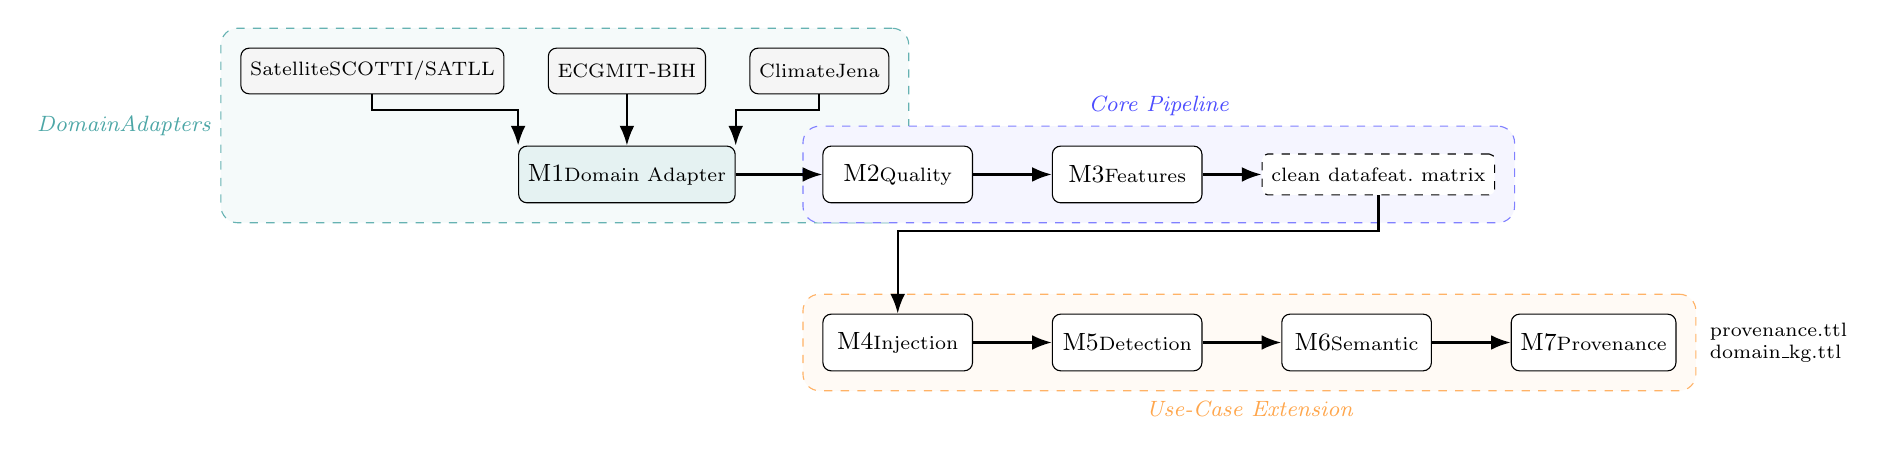
\begin{tikzpicture}[
  box/.style={draw, rounded corners=3pt, minimum width=1.9cm, minimum height=0.72cm,
              text centered, font=\small, fill=white},
  src/.style={draw, rounded corners=3pt, minimum width=1.6cm, minimum height=0.58cm,
              text centered, font=\scriptsize, fill=gray!8},
  art/.style={draw, dashed, rounded corners=2pt, minimum width=1.7cm,
              minimum height=0.52cm, text centered, font=\scriptsize, fill=white},
  arr/.style={-{Latex[length=2.5mm]}, thick},
  node distance=1.0cm
]
%% --- Domain inputs (top row) ---
\node[src] (sat) {Satellite\\[-1pt]\scriptsize SCOTTI/SATLL};
\node[src, right=0.55cm of sat] (ecg) {ECG\\[-1pt]\scriptsize MIT-BIH};
\node[src, right=0.55cm of ecg] (clim) {Climate\\[-1pt]\scriptsize Jena};

%% --- M1 adapter below inputs ---
\node[box, below=0.65cm of ecg, fill=teal!10] (m1) {M1\\[1pt]\scriptsize Domain Adapter};
\draw[arr] (sat.south)  -- ++(0,-0.2) -| (m1.north west);
\draw[arr] (ecg.south)  -- (m1.north);
\draw[arr] (clim.south) -- ++(0,-0.2) -| (m1.north east);

%% --- Core pipeline (M2, M3) ---
\node[box, right=1.1cm of m1] (m2) {M2\\[1pt]\scriptsize Quality};
\node[box, right=of m2]       (m3) {M3\\[1pt]\scriptsize Features};
\node[art, right=0.75cm of m3] (clean) {clean data\\feat.\ matrix};
\draw[arr] (m1) -- (m2);
\draw[arr] (m2) -- (m3);
\draw[arr] (m3) -- (clean);

%% --- Use-case extension (M4-M7, bottom row) ---
\node[box, below=1.4cm of m2] (m4) {M4\\[1pt]\scriptsize Injection};
\node[box, right=of m4]       (m5) {M5\\[1pt]\scriptsize Detection};
\node[box, right=of m5]       (m6) {M6\\[1pt]\scriptsize Semantic};
\node[box, right=of m6]       (m7) {M7\\[1pt]\scriptsize Provenance};
\draw[arr] (m4) -- (m5);
\draw[arr] (m5) -- (m6);
\draw[arr] (m6) -- (m7);
\draw[arr] (clean.south) -- ++(0,-0.45) -| (m4.north);

%% --- Output label ---
\node[right=0.3cm of m7, align=left, font=\scriptsize]
  {provenance.ttl\\domain\_kg.ttl};

%% --- Bounding boxes ---
\begin{scope}[on background layer]
  \node[draw=teal!60, dashed, rounded corners=6pt, fill=teal!4, inner sep=7pt,
        fit={(sat)(ecg)(clim)(m1)},
        label={[font=\footnotesize\itshape,text=teal!70]left:{Domain\\Adapters}}] {};
  \node[draw=blue!50, dashed, rounded corners=6pt, fill=blue!4, inner sep=7pt,
        fit={(m2)(m3)(clean)},
        label={[font=\footnotesize\itshape,text=blue!70]above:{Core Pipeline}}] {};
  \node[draw=orange!60, dashed, rounded corners=6pt, fill=orange!4, inner sep=7pt,
        fit={(m4)(m5)(m6)(m7)},
        label={[font=\footnotesize\itshape,text=orange!70]below:{Use-Case Extension}}] {};
\end{scope}
\end{tikzpicture}
\caption{SensorWF architecture. Three domain adapters (teal) standardise inputs
         from satellite telemetry, ECG, and climate data into a common DataFrame schema.
         The core pipeline (blue, M2--M3) performs quality assessment and feature engineering.
         The use-case extension (orange, M4--M7) runs fault injection, ML anomaly detection,
         semantic annotation, and PROV-O/ProvONE provenance export -- identical across all domains.}
\label{fig:architecture}
\end{figure*}

%% Fig 2 -- Cross-domain comparison
\begin{figure}[t]
\centering

\includegraphics[width=\columnwidth]{../../results/figures/fig_domain_comparison.png}
\caption{Cross-domain detection performance across satellite (SATLL), biomedical ECG
         (MIT-BIH), and atmospheric climate (Jena) domains. Each panel shows one metric
         (Recall, FPR, F1, AUC-ROC) grouped by domain and coloured by detector.
         Values are averaged over all sessions per domain. AE = Autoencoder,
         IF = IsolationForest, RRZS = RobustRollingZScore, ZS = ZScore.}
\label{fig:crossdomain}
\end{figure}

%% Fig 3 -- Satellite telemetry dashboard
\begin{figure}[t]
\centering
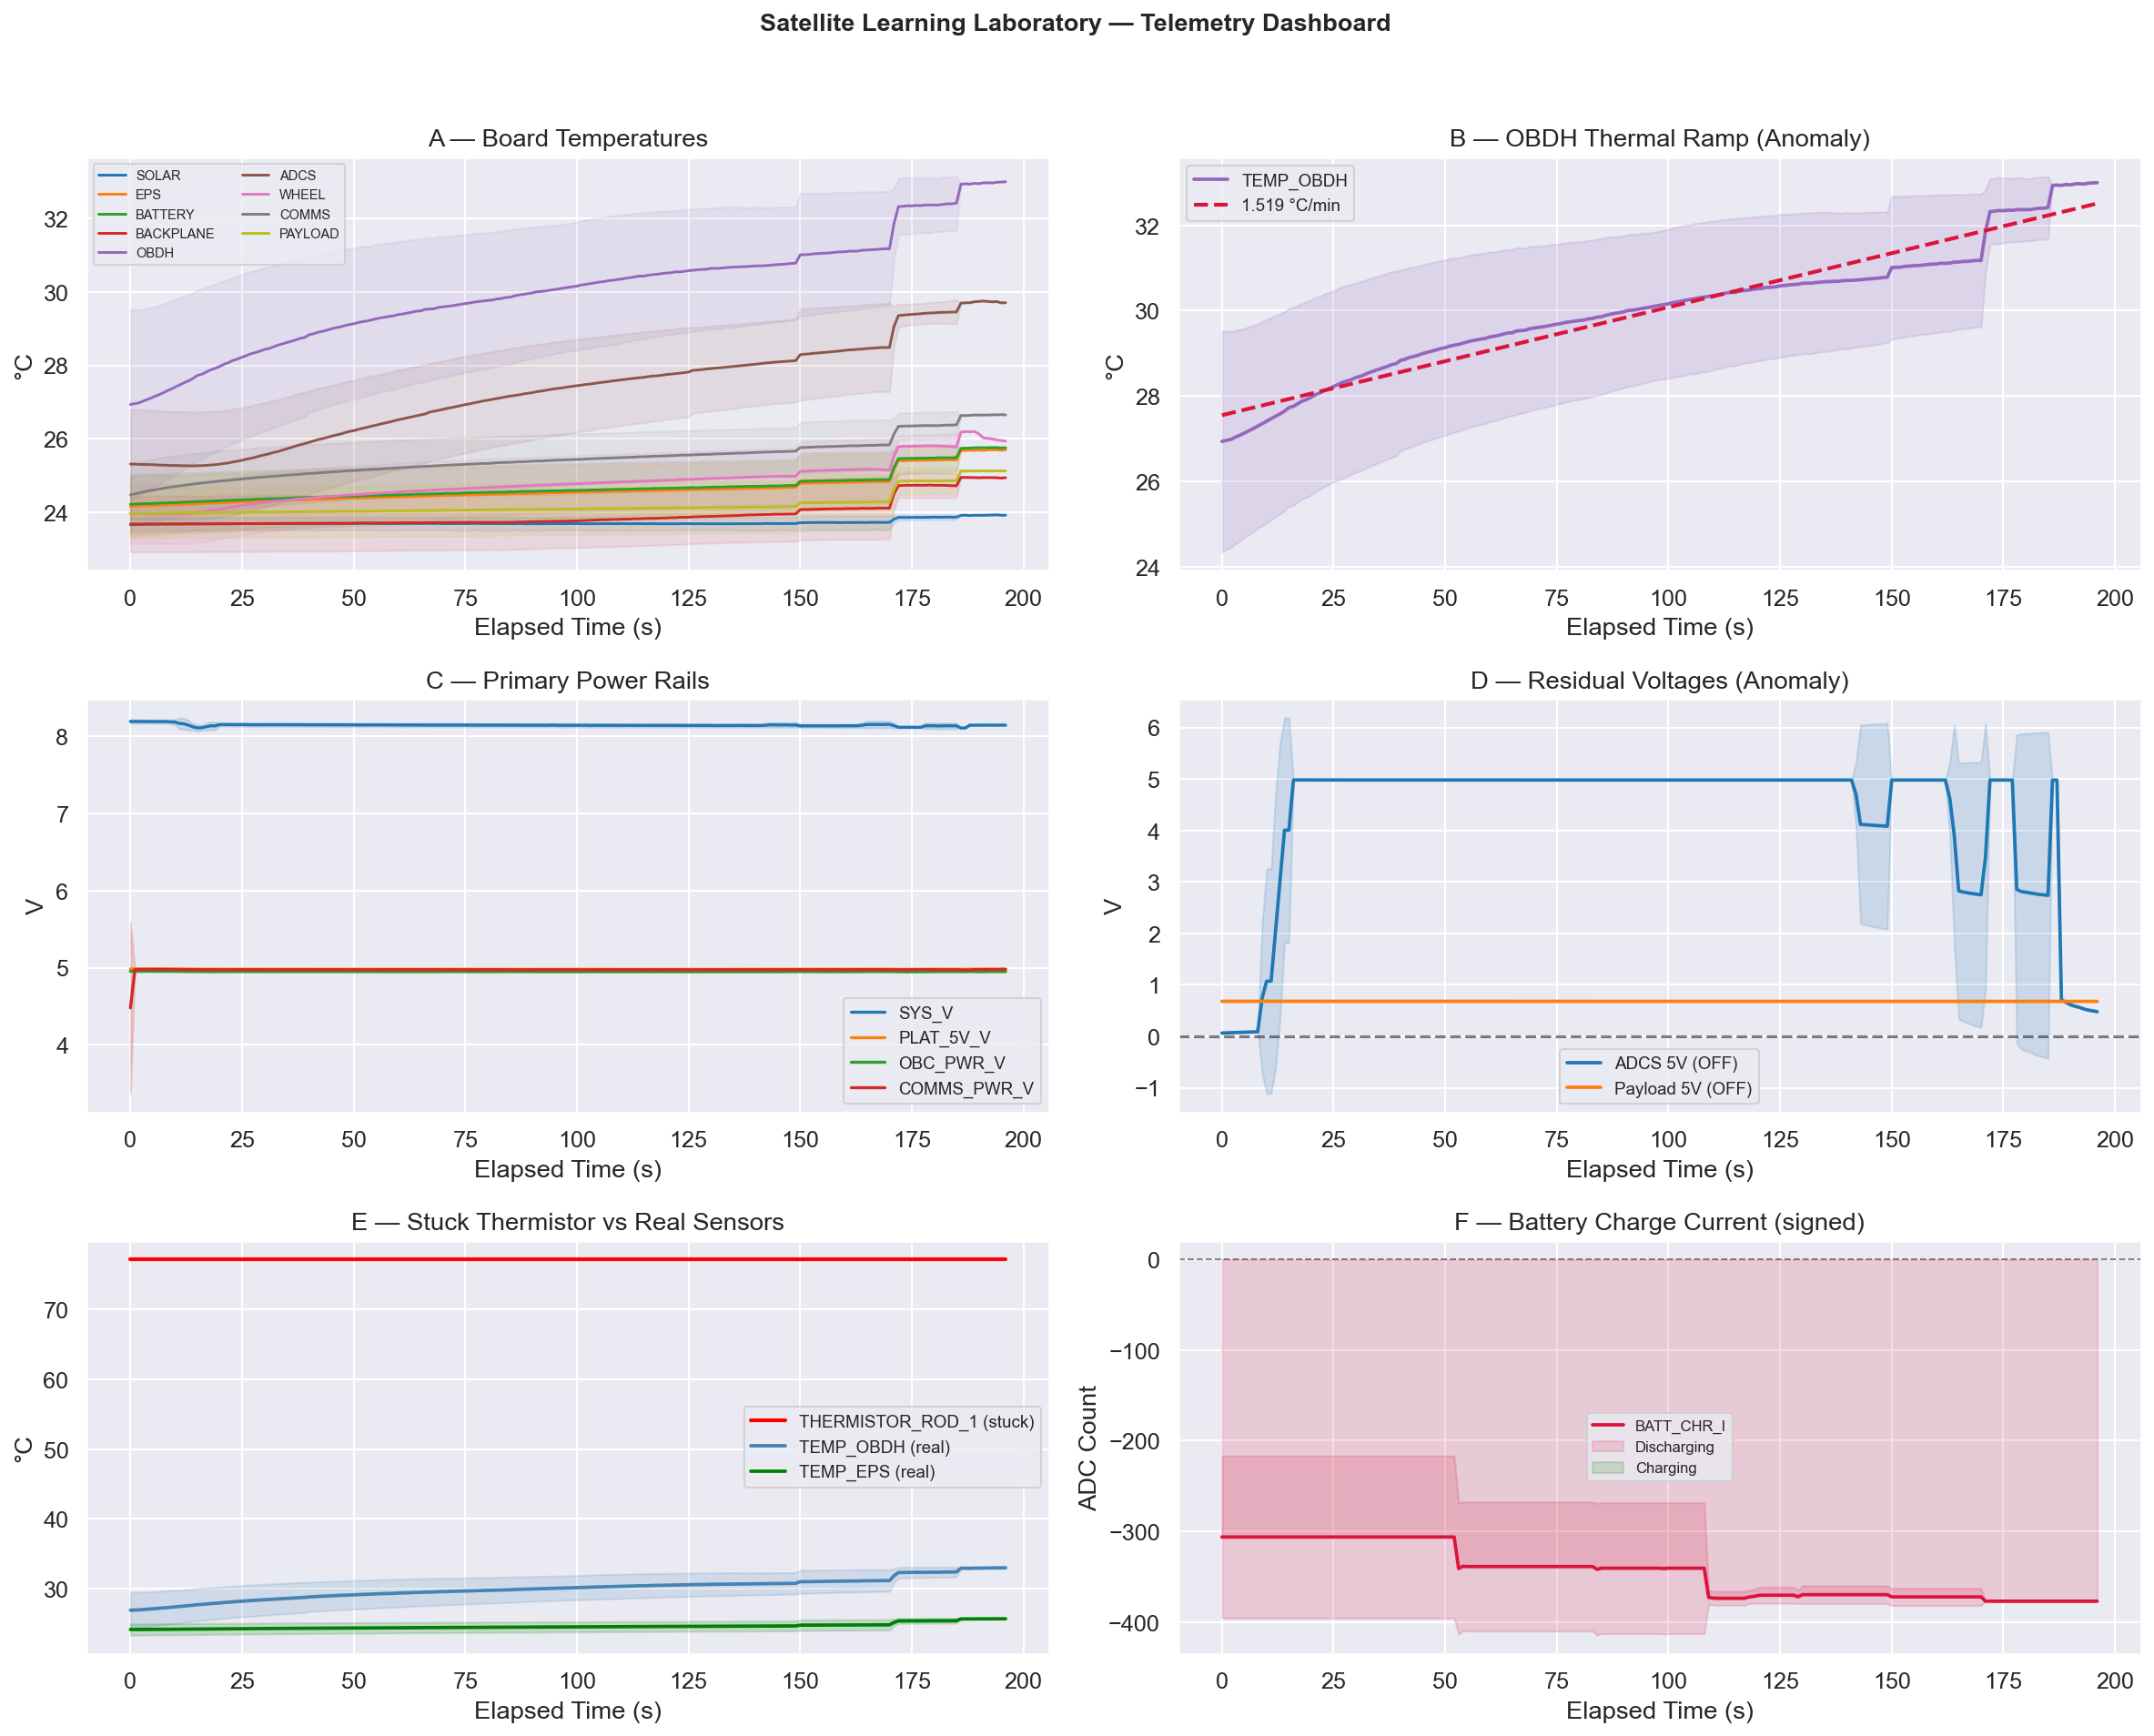
\includegraphics[width=\columnwidth]{../../results/AccelerometerTest/07_summary_dashboard.png}
\caption{AccelerometerTest telemetry summary (M2/M3, satellite domain). The OBDH
         thermal ramp ($+0.68\,^{\circ}$C/min, $R^2\!=\!0.86$) is the dominant
         clean-data feature and primary confound for thermal fault injection by M4.
         Z-score flags on power rails (\texttt{PLAT\_5V\_V}, \texttt{SYS\_V}) are
         recorded as \texttt{sensorwf:hasAssumption} predicates in the provenance trace.}
\label{fig:dashboard}
\end{figure}

%% Fig 4 -- Provenance graph
\begin{figure}[t]
\centering
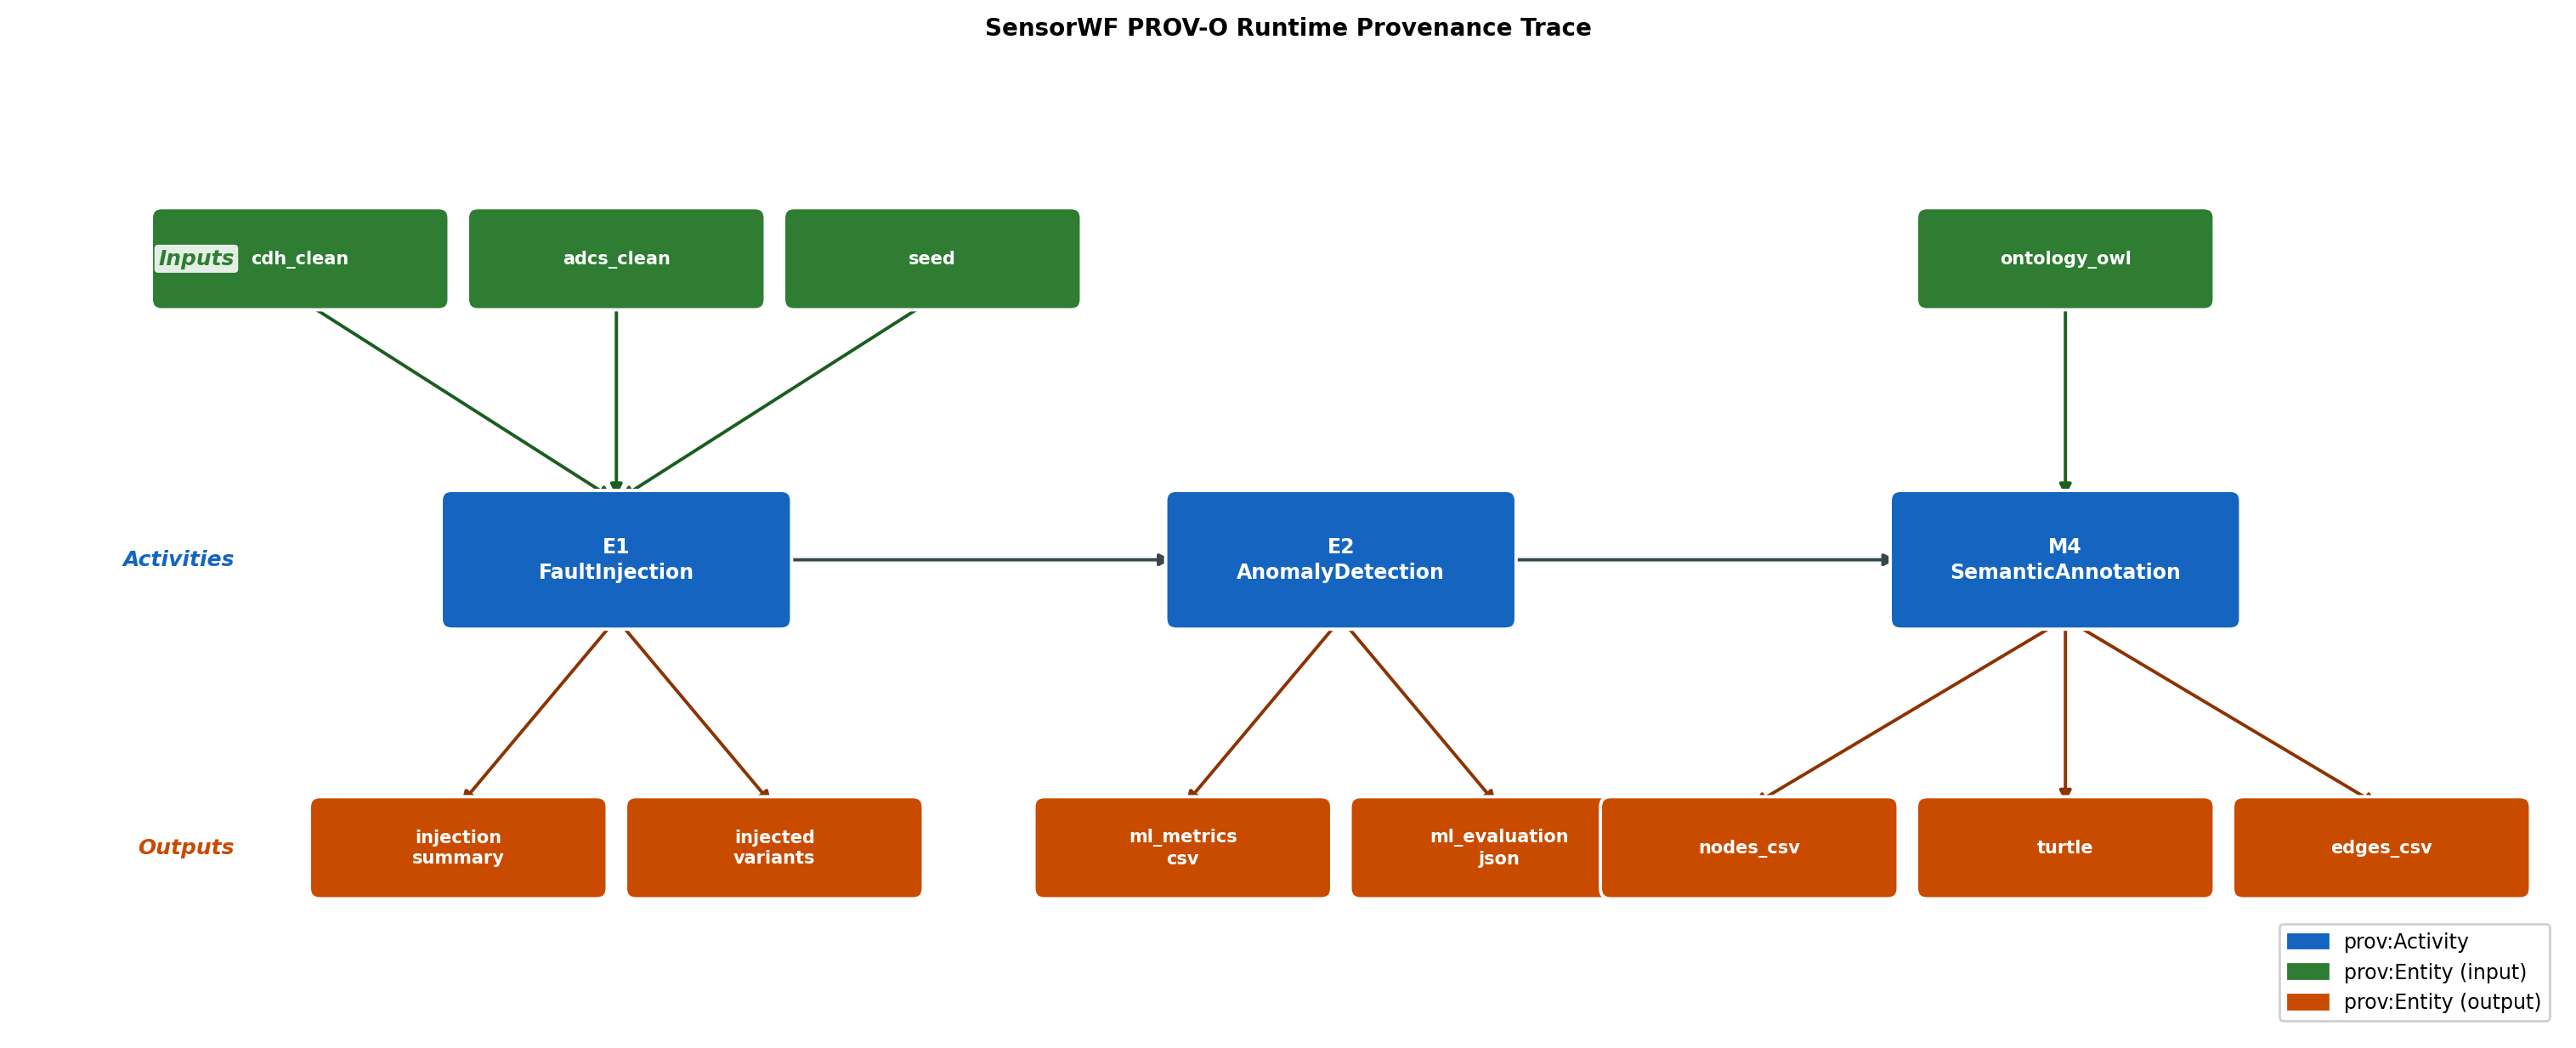
\includegraphics[width=\columnwidth]{../../results/figures/fig_provenance.png}
\caption{Runtime provenance graph for the satellite use-case extension (M4--M7),
         rendered from \texttt{provenance.ttl}. Blue squares are \texttt{prov:Activity}
         nodes (module executions); orange circles are \texttt{prov:Entity} nodes
         (data artefacts). Edges encode \texttt{prov:used} and
         \texttt{prov:wasGeneratedBy} relations. The same provenance structure is
         emitted for ECG and climate domain runs.}
\label{fig:provenance}
\end{figure}

%% Fig 5 -- Semantic KG subgraph
\begin{figure}[t]
\centering
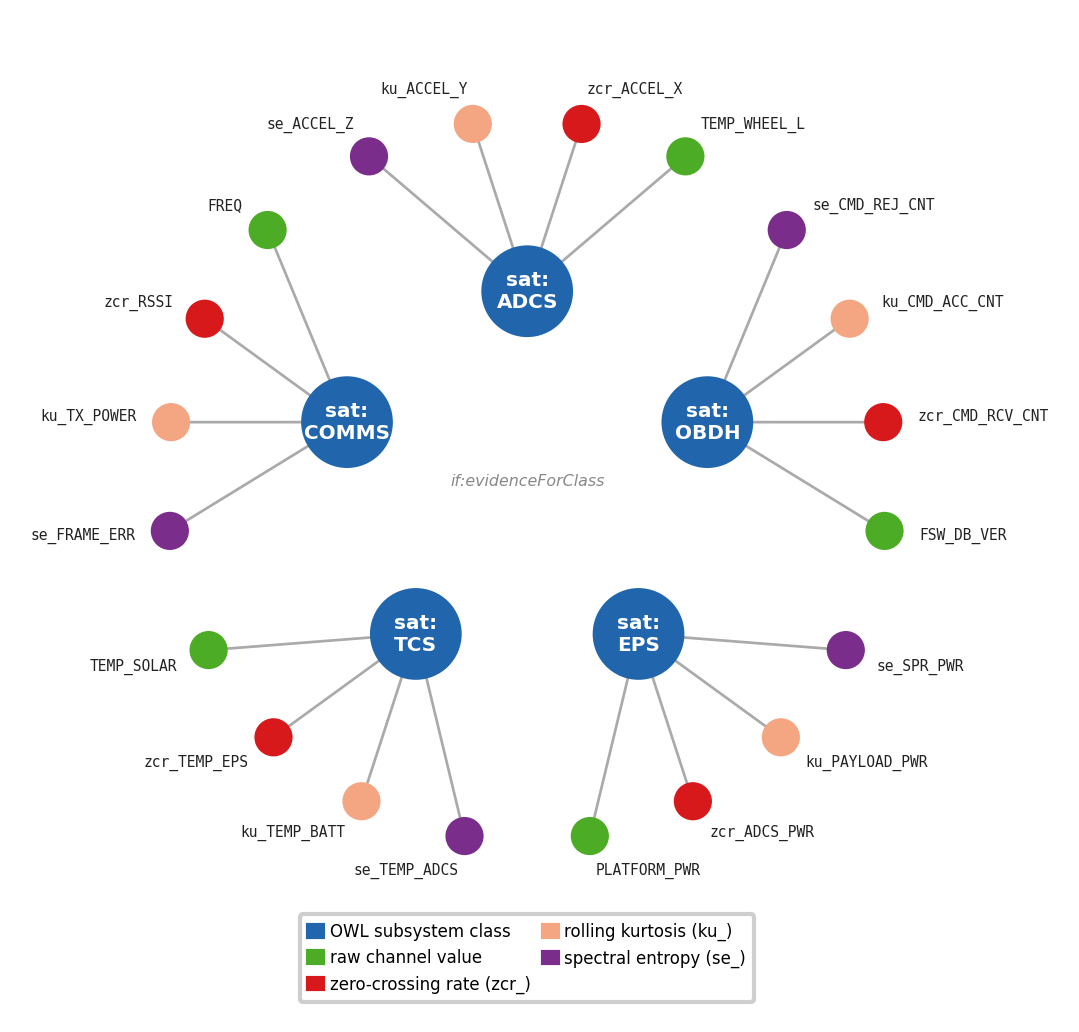
\includegraphics[width=\columnwidth]{../../results/figures/fig_kg_subgraph.png}
\caption{Subgraph of the satellite ontology-linked knowledge graph produced by M6
         (full graph: 765 nodes, 12,209 edges). Red nodes are OWL class instances
         from the satellite ontology; blue nodes are feature nodes; green nodes are
         per-instance anomaly instances. Edges encode IsolationForest feature importance
         and ontology evidence relations. Equivalent graphs are produced for ECG
         (\texttt{ecg.owl}) and climate (\texttt{climate.owl}) domains.}
\label{fig:kgsubgraph}
\end{figure}

\end{document}
